\section{Results}

% ------------------------------------------------------------------------------
\begin{frame}{Debiasing removes the template shortcuts}
  \begin{columns}[c]
    \begin{column}{0.56\textwidth}
      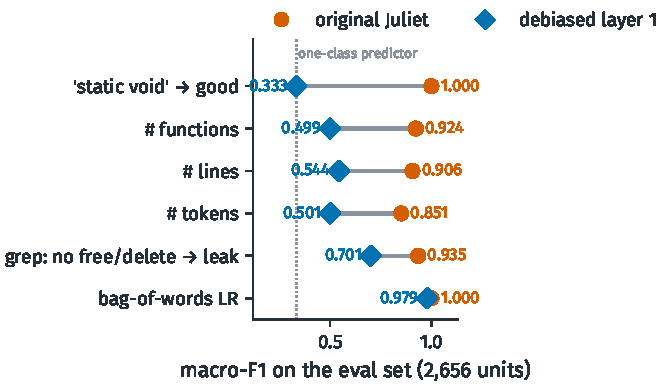
\includegraphics[width=\linewidth]{figures/probes.pdf}
    \end{column}
    \begin{column}{0.42\textwidth}
      \begin{itemize}
        \item Format cues fall to chance
        \item \code{static void}: \res{x}{probe_static_void_original} $\to$ \res{x}{probe_static_void_layer1}
        \item grep: \res{grep-original}{macro} $\to$ \res{grep-layer1}{macro}
        \item Bag-of-words: task words only
      \end{itemize}
    \end{column}
  \end{columns}
  \vfill
  {\scriptsize Probes fitted on dev, scored on eval. Bag-of-words cues: \code{free}, \code{delete}, \code{ALLOCA}.\par}
\end{frame}

% ------------------------------------------------------------------------------
\begin{frame}{The three best detectors on Debiased are LLM-based}
  \centering
  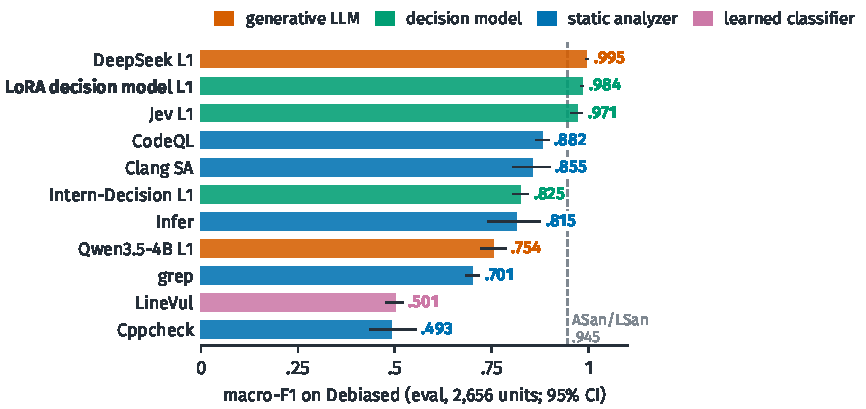
\includegraphics[width=0.86\linewidth,height=0.74\textheight,keepaspectratio]{figures/quality.pdf}\\[2pt]
  Best static analyzer: CodeQL \res{codeql-layer1}{macro}; best LLM: DeepSeek L1 \res{deepseek_L1-layer1}{macro}
\end{frame}

% ------------------------------------------------------------------------------
% src (paired bootstrap): parent analysis juliet_full/analysis/near_llm_bootstrap.py, seed 20261123, B=2000 family-cluster resamples,
%   n=2,656 Debiased eval units, macro-F1 difference; LoRA L1 - DeepSeek L1 = -0.0113 [-0.0143, -0.0084]
%   (12 vs 42 units only-right); LoRA L1 - Jev L1 = +0.0132 [0.0029, 0.0282].
% Margin 0.02: pre-registered near-LLM criterion, PLAN.md section 4.2.
\begin{frame}{Our decision model is 1.1 points below DeepSeek, above Jev}
  \centering
  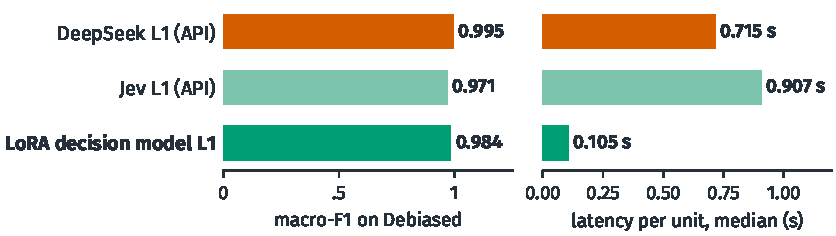
\includegraphics[width=0.92\linewidth]{figures/nearllm.pdf}
  \vspace{4pt}
  \begin{itemize}
    \item vs DeepSeek: $\Delta = -0.011$, 95\% CI $[-0.014, -0.008]$
    \item Inside our pre-registered 0.02 margin
    \item vs Jev: $\Delta = +0.013$, 95\% CI $[+0.003, +0.028]$
  \end{itemize}
\end{frame}

% ------------------------------------------------------------------------------
\begin{frame}{About 7$\times$ faster than DeepSeek, at the IDE budget edge}
  \centering
  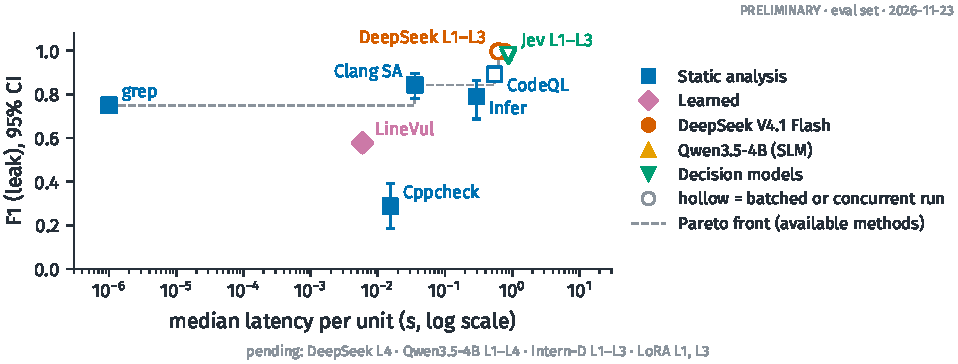
\includegraphics[width=\linewidth,height=0.72\textheight,keepaspectratio]{figures/pareto.pdf}\\[2pt]
  LoRA decision model 0.105\,s vs DeepSeek 0.715\,s per unit; no API cost
\end{frame}

% ------------------------------------------------------------------------------
\begin{frame}{DeadFree breaks learned models in two opposite ways}
  \centering
  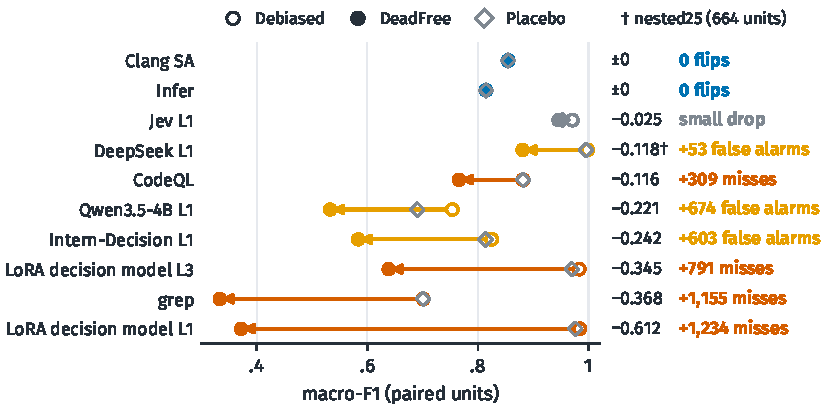
\includegraphics[width=0.88\linewidth,height=0.66\textheight,keepaspectratio]{figures/deadfree.pdf}\\[2pt]
  {\small\textcolor{OIvermil}{\textbf{Misses}}: any \code{free} means freed \quad
  \textcolor{OIorange}{\textbf{False alarms}}: guarded real \code{free} doubted\par}
  {\scriptsize Placebo barely moves: the drop comes from the dead free.\par}
\end{frame}

% ------------------------------------------------------------------------------
\begin{frame}{Fine-tuning learned the free-shortcut}
  \begin{columns}[c]
    \begin{column}{0.52\textwidth}
      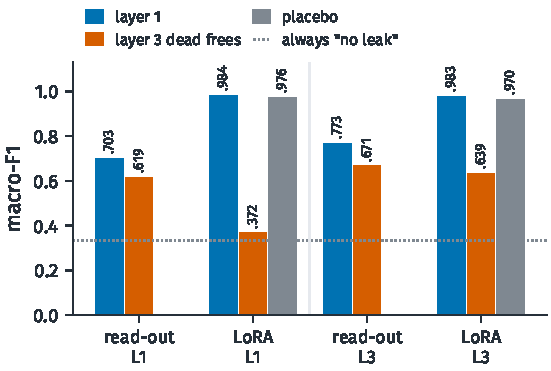
\includegraphics[width=\linewidth]{figures/lora.pdf}
    \end{column}
    \begin{column}{0.46\textwidth}
      \begin{itemize}
        \item L1: \res{lora_L1-layer1}{macro} $\to$ \alert{\res{lora_L1-layer3}{macro}} on DeadFree
        \item Leak recall: \alert{\res{lora_L1-layer3}{r}}
        \item No LoRA: \res{readout_L1-layer1}{macro} $\to$ \res{readout_L1-layer3}{macro}
        \item Placebo \res{lora_L1-placebo}{macro}: cue is \code{free}
      \end{itemize}
    \end{column}
  \end{columns}
  \vfill
  {\small Training sharpened ``\code{free} present $\Rightarrow$ safe''.\par}
\end{frame}

% ------------------------------------------------------------------------------
\begin{frame}{Clang SA evidence (L3) helps weak models most}
  \centering
  \renewcommand{\arraystretch}{1.15}
  \begin{tabular}{@{}lcccc@{}}
    \toprule
    & \multicolumn{2}{c}{Debiased} & \multicolumn{2}{c}{DeadFree} \\
    \cmidrule(lr){2-3}\cmidrule(l){4-5}
    Model & L1 & L3 & L1 & L3 \\
    \midrule
    Qwen3.5-4B & \res{qwen_L1-layer1}{macro} & \textbf{\res{qwen_L3-layer1}{macro}} & \res{qwen_L1-layer3}{macro} & \textbf{\res{qwen_L3-layer3}{macro}} \\
    Intern-Decision & \res{intern_L1-layer1}{macro} & \textbf{\res{intern_L3-layer1}{macro}} & \res{intern_L1-layer3}{macro} & \textbf{\res{intern_L3-layer3}{macro}} \\
    LoRA decision model & \res{lora_L1-layer1}{macro} & \res{lora_L3-layer1}{macro} & \res{lora_L1-layer3}{macro} & \textbf{\res{lora_L3-layer3}{macro}} \\
    DeepSeek & \res{deepseek_L1-layer1}{macro} & \res{deepseek_L3-layer1}{macro} & \res{deepseek_L1-layer3}{macro}$^\dagger$ & \res{deepseek_L3-layer3}{macro}$^\dagger$ \\
    \bottomrule
  \end{tabular}
  \vspace{8pt}

  No gain at the top; +0.05 to +0.27 below it\\[2pt]
  {\scriptsize Macro-F1. $^\dagger$\,DeepSeek DeadFree: nested25 subset (664 units).\par}
\end{frame}

% ------------------------------------------------------------------------------
\begin{frame}{Path-sensitive analyzers ignore dead frees}
  \centering
  \renewcommand{\arraystretch}{1.15}
  \begin{tabular}{@{}lccc@{}}
    \toprule
    Tool & Debiased & DeadFree & flips \\
    \midrule
    Clang SA & \res{clang_sa-layer1}{macro} & \res{clang_sa-layer3}{macro} & \res{clang_sa-layer3}{flips} \\
    Infer & \res{infer-layer1}{macro} & \res{infer-layer3}{macro} & \res{infer-layer3}{flips} \\
    Cppcheck & \res{cppcheck-layer1}{macro} & \res{cppcheck-layer3}{macro} & \res{cppcheck-layer3}{flips} \\
    Dynamic-enhanced & \res{dynamic_enhanced-layer1}{macro} & \res{dynamic_enhanced-layer3}{macro} & \res{dynamic_enhanced-layer3}{flips} \\
    \bottomrule
  \end{tabular}
  \vspace{8pt}
  \begin{itemize}
    \item They prune the infeasible branch
    \item Robust, but Clang SA recall is only \res{clang_sa-layer1}{r}
  \end{itemize}
\end{frame}

% ------------------------------------------------------------------------------
\begin{frame}[fragile]{Live: one dead free fools grep and our model}
  \begin{columns}[T]
    \begin{column}{0.54\textwidth}
      {\small Bad unit \texttt{strdup\_char\_01}, plus:\par}
\begin{lstlisting}[style=unit]
static const int sym_61 = 4;
...
data = strdup(myString);
printLine(data);
(*\hlc{if(sym\_61 > 4) \{ free(data); \}}*)
\end{lstlisting}
      {\small The free never runs: still a leak.\par}
    \end{column}
    \begin{column}{0.44\textwidth}
      \textcolor{OIvermil}{\textbf{Flips to ``safe''}}
      \begin{itemize}
        \item grep, LoRA decision model
      \end{itemize}
      \vspace{4pt}
      \textcolor{OIblue}{\textbf{Still ``leak''}}
      \begin{itemize}
        \item Clang SA, DeepSeek, Jev
      \end{itemize}
    \end{column}
  \end{columns}
  \vfill
  {\scriptsize Backup: \texttt{demo/recordings/stage\_final.mp4}; \texttt{demo.py --replay recordings/stage\_final.json}.\par}
\end{frame}
